\clearpage
\subsection{Subsistema de audio}

El subsistema analógico de audio tiene tres funciones principales:
\begin{enumerate}
    \item Multiplexar las dos entradas de audio (MP3 y Radio) a un ADC del microcontrolador
    \item Multiplexar la salida proveniente del DAC a una de las dos salidas de audio (Altavoces o auriculares)
    \item Amplificar la salida de audio seleccionada
\end{enumerate}

\subsubsection{Divisor de rail}
Este sistema se alimenta directamente desde el módulo de alimentación explicado en el apartado anterior. Por ello, cuenta con una entrada unipolar de 7 voltios. Sin embargo, los circuitos de audio necesitan alimentación bipolar para funcionar. Por ello, hemos decidido implementar un circuito divisor de rail, que genera una tensión intermedia que se utilizará como nueva referencia del circuito, obteniendo una alimentación virtual de $\pm$3.5 V.

El circuito utilizado es un divisor de tensión de precisión implementado mediante el amplificador operacional \texttt{OP07}. Este amplificador operacional tiene muy bajo error estático y además cuenta con dos terminales para el ajuste del offset mediante un potenciómetro, por lo que es ideal para nuestra aplicación.

Sin embargo, los amplificadores operacionales permiten muy poca corriente a través de su terminal de salida, por lo que se necesita un circuito que permita incrementar la corriente de salida o entrada de dicho circuito sin afectar demasiado a la salida. Para ello, se utiliza una topología \textit{Push-Pull} en la que se utilizan dos pares de Darlington, es decir, cuatro transistores, para incrementar la capacidad de corriente del circuito. 

Al introducirlos dentro del lazo de realimentación, se elimina el efecto de las tensiones de base y se elimina el ruido que pudieran introducir, pero a cambio introducen la posibilidad de inestabilizar el circuito. Teniendo esta posibilidad en cuenta, incluimos la posibilidad de soldar un condensador entre el terminal de salida del amplificador y la alimentación negativa del circuito, para introducir un polo que compense la estabilidad. Sin embargo, hemos acabado no necesitando utilizarlo. 

Por tanto, el circuito generador de tierra virtual o divisor de rail queda como se puede ver en la \autoref{fig:2-2-tierra-virtual}.

\begin{figure}[h]
    \centering
    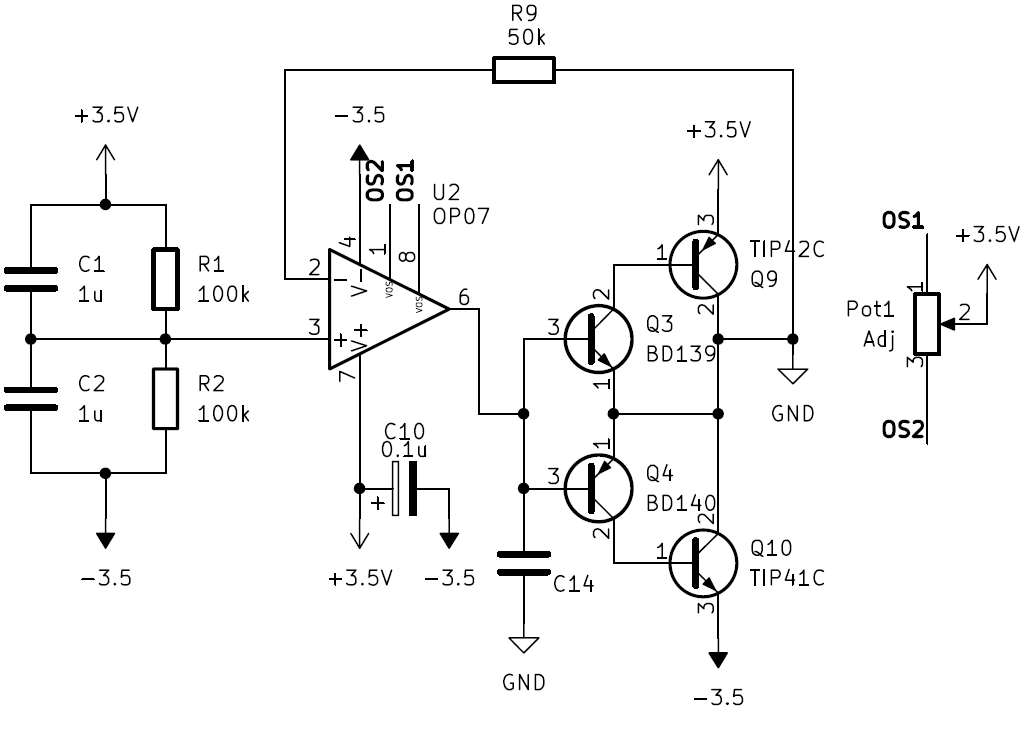
\includegraphics[width=0.5\textwidth]{images/2/2-2/circuitoDivisorRail.png}
    \caption{Circuito divisor de raíl}
    \label{fig:2-2-tierra-virtual}
\end{figure}

\subsubsection{Habilitación del circuito}

Para eliminar el consumo parásito del circuito cuando el sistema entre en el modo bajo consumo, se ha implementado un subcircuito de habilitación el cual permite encender o apagar el resto de subsistema (aunque finalmente el consumo parásito es muy pequeño).

Dicho circuito consiste en un transistor MOSFET de canal N en la alimentación, que permite cortar o dejar pasar la alimentación. Además, la baja impedancia de conducción del transistor permite que no haya casi pérdidas de potencia en el transistor. Sin embargo, ya que para cortar el transistor se necesita polarizar la puerta con una tensión próxima a 7 voltios y soportar las corrientes de los transitorios de conmutación, se utiliza otro transistor con una resistencia de \textit{pull-up} para adaptar los niveles los GPIO y reducir la corriente necesaria. Esto tiene el efecto añadido de invertir la polaridad de la habilitación que junto a la inversión del canal N se anulan, provocando que un nivel alto en el GPIO habilite el circuito. 

Por tanto, el circuito final es el que se ve en la \autoref{fig:2-2-circuito-habilitacion}.

\begin{figure}[h]
    \centering
    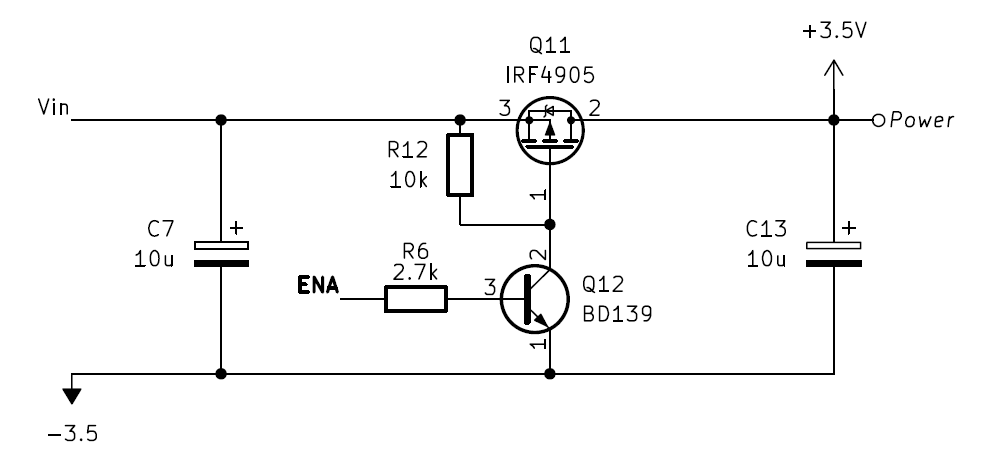
\includegraphics[width=0.5\textwidth]{images/2/2-2/circuitoHabilitacion.png}
    \caption{Circuito de habilitación}
    \label{fig:2-2-circuito-habilitacion}
\end{figure}

\subsubsection{Multiplexación de audio}

Para la multiplexación de audio se va a utilizar un multiplexor integrado. Inicialmente tratamos de diseñar un circuito que multiplexara los caminos de audio mediante componentes discretos, encontrando la estructura de la Puerta de Transmisión \cite{TransmissionGate}, como la que se puede ver en la \autoref{fig:2-2-puerta-transmision}

Sin embargo, todas las estructuras discretas que encontramos necesitan una familia de transistores de efecto de campo en los que el canal no está unido internamente al sustrato, permitiendo cargar la capacidad puerta-canal sin afectar a la tensión del camino drenador-surtidor. 

El principal problema de estos transistores es su elevado precio y muy poca variedad, siendo casi imposible encotrarlos. Además, generalmente se utilizan en aplicaciones de alta potencia por lo que su rendimiento para aplicaciones de baja señal suele ser bastante pobre.

\begin{figure}[h]
    \centering
    \includegraphics[width=0.3\textwidth]{images/2/2-2/puertaTransmisión.png}
    \caption{Puerta de transmisión con transistores con canal desconectado}
    \label{fig:2-2-puerta-transmision}
\end{figure}

Finalmente, descartamos la idea de utilizar componentes discretos y utilizamos una solución integrada. Por tanto, utilizamos el multiplexor analógico \texttt{CD4053BC}. \cite{CD4053BDataSheet}

Este multiplexor cuenta con tres canales en configuración \texttt{SPDT}, por lo que cada canal tiene un terminal en un extremo y dos en el otro. Este multiplexor cuenta con la ventaja de ser bidireccional, cosa de la que muchos otros carecen y es fundamental para nuestra funciononalidad.

Este multiplexor se utiliza para conectar las dos entradas de audio, que provienen de conectores Jack de audio de 3.5 mm a un GPIO que se conecta internamente a un ADC de la placa y para conectar otro GPIO que se conecta internamente a un DAC a las entradas de los dos caminos de amplificación de audio. 

\subsubsection{Cambiador de nivel lógico}

Un error que cometimos es no tener en cuenta la tensión de habilitación necesaria para conmutar un canal del multiplexor, por lo que los 3.3V de salida de un GPIO no son suficientes para cambiar el canal del multiplexor. Esto provoca que se esté siempre seleccionado el canal correspondiente al nivel bajo.

Para solucionar esto, hemos construido un circuito cambiador de nivel lógico que adapta los 3.3 V de la placa a los 7 V necesarios para conmutar el multiplexor (realmente el mínimo es aproximadamente 5V).

La solución que hemos pensado consiste en un inversor lógico TTL, que consiste en un transistor bipolar NPN con una resistencia de \textit{Pull-up}. La única desventaja es la inversión de nivel, pero se corrige fácilmente en el software.

Se puede ver el diagrama de nuestra solución en la \autoref{fig:2-2-cambiador-nivel}, en la que se muestra un cambiador. Hemos soldado dos de ellos en una placa de prototipado, que se puede ver en la \autoref{fig:2-2-foto-cambiador}.

\begin{figure}[h]
    \centering
    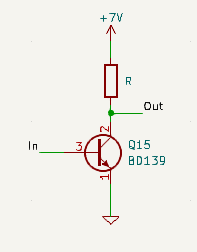
\includegraphics[width=0.5\textwidth]{images/2/2-2/circuitoCambiadorNivel.png}
    \caption{Circuito cambiador de niveles}
    \label{fig:label}
\end{figure}

\begin{figure}[h]
    \centering
    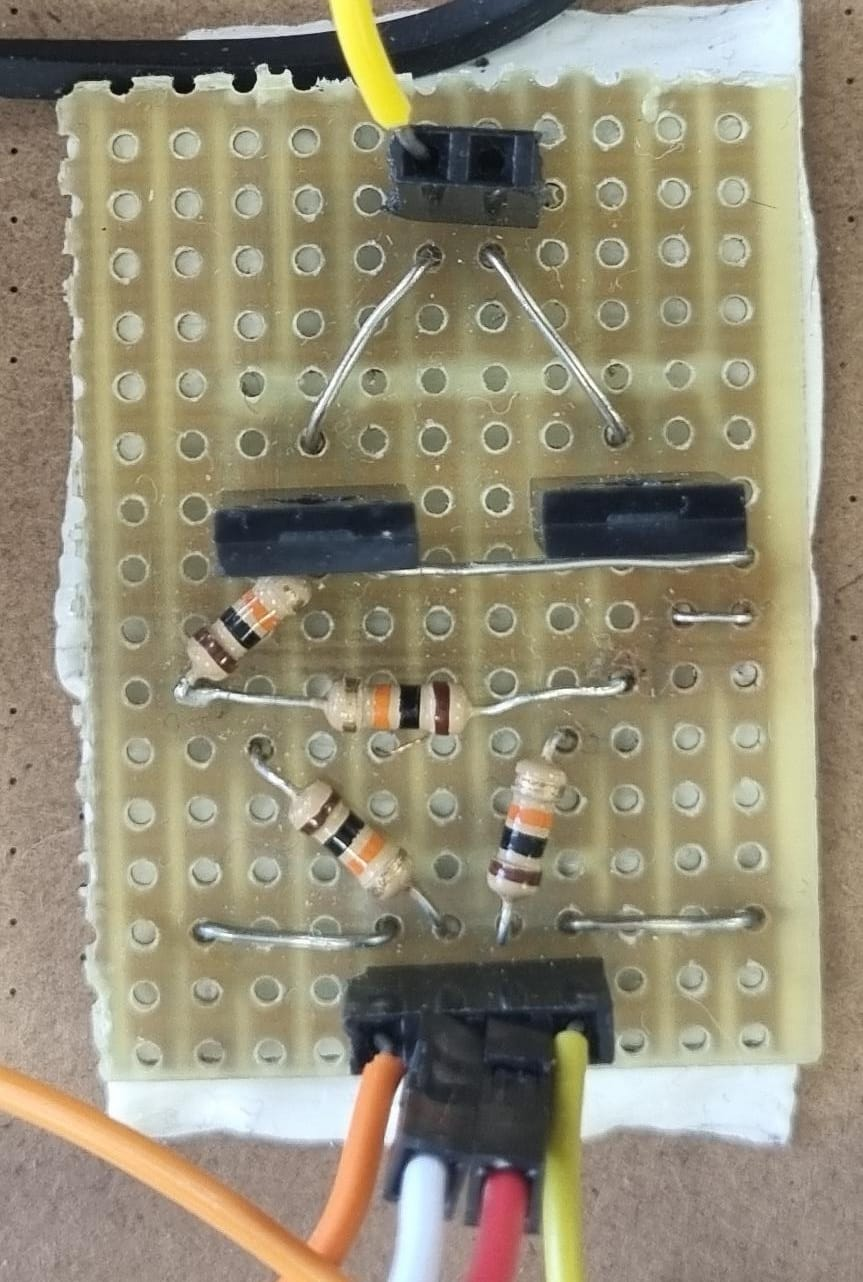
\includegraphics[width=0.25\textwidth]{images/2/2-2/cambiadorNivel.jpg}
    \caption{Foto del circuito cambiador de nivel}
    \label{fig:2-2-foto-cambiador}
\end{figure}
\subsubsection{Amplificador de audio para los auriculares}

La salida del DAC de la placa es una señal entre 0 y 3.3 V con 12 bits de resolución. Por tanto, el audio que se genere tiene una componente continua que se debe eliminar. 

Para eliminar esta componente continua hemos implementado una configuración de filtro paso alto mediante un filtrado pasivo y un seguidor de tensión realizado con un amplificador operacional. En el camino de realimentación del amplificador operacional se coloca una resistencia para anular la tensión de error de \textit{offset} del amplificador operacional.

También se añade la misma estructura de transistores que en el circuito generador de tierra virtual, que ahora al estar también dentro del lazo de realimentación cuentan con la ventaja de que se anula la distorsión de cruce. 

Los valores elegidos para los componentes del filtro son una resistencia de $100\ k\Omega$ y un condensador de $100\ nF$. Con ello, conseguimos una frecuencia de corte de:

\[
    f_c = \frac{1}{2\pi RC} \approx 16\ Hz    
\]

Elegimos este valor ya la banda de audición humana máxima es de $20$ Hz a $20$ kHz.

Se puede ver un diagrama de la solución que montamos en la \autoref{fig:2-2-amp-cascos}.

\begin{figure}[h]
    \centering
    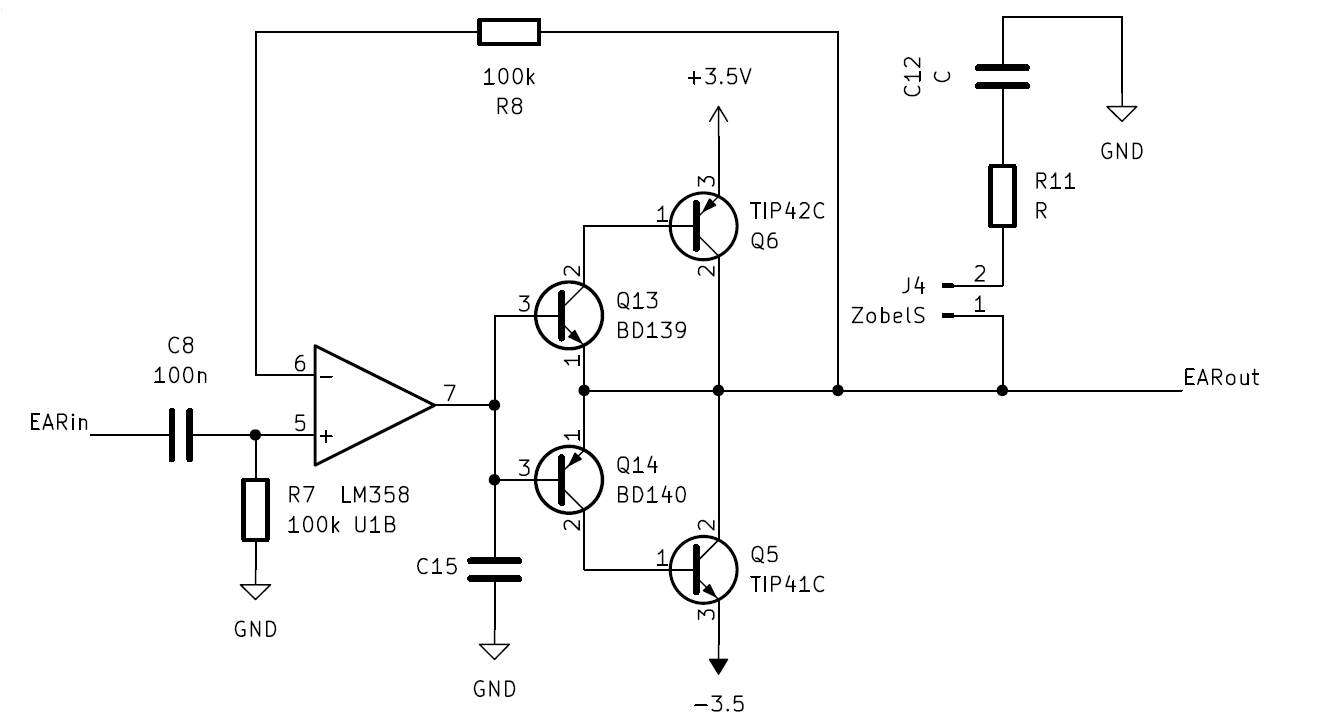
\includegraphics[width=0.7\textwidth]{images/2/2-2/circuitoAmplificadorCascos.png}
    \caption{Circuito amplificador de auriculares}
    \label{fig:2-2-amp-cascos}
\end{figure}

Sin embargo, al montar y probar el circuito detectamos que tenía un problema de inestabilidad para una frecuencia, lo cual es un problema común en los circuitos realimentados. Esto ocurre ya que la introducción del los transistores añade modificaciones impredecibles a la ganancia de lazo, provocando un muy molesto zumbido en los altavoces.

La solución que encontramos a este problema es la realimentación parcial mediante un condensador entre la salida del amplificador operacional y la base de los transistores. El tamaño del condensador afecta directamente a la reducción del ruido, cuanta más capacidad mejor lo elimina ya que hace una realimentación más directa. Sin embargo, cuanta mayor capacidad se le aplique, más se aprecia el efecto de la distorsión de cruce, la cual era eliminada al hacer la realimentación a la salida.

Experimentalmente probamos valores distintos determinando que el mejor balance entre ruido y distorsión de cruce se tiene para un valor aproximado de $33 \mu F$. Sin embargo, este valor no es propio del circuito sino de las tolerancias y efectos parásitos de los componentes, por lo que podría variar mucho según las circunstancias.

Otra cuestión a la que nos enfrentamos es la cantidad de canales. Inicialmente diseñamos el circuito para ofrecer un solo canal de audio y dirigirlo a ambos canales, pero se pierde bastante calidad por lo que decidimos dejarlo en audio por un solo canal. Si se quisiera obtener audio por ambos canales o incluso estéreo, se debería duplicar este circuito y colocar uno por canal.

\subsubsection{Amplificador de altavoces}

El circuito amplificador de altavoces cuenta con el mismo paso bajo que el amplificador de los auriculares, pero se utiliza otra resistencia para aportar ganancia al circuito. Además, ya que se introduce la rama a tierra se añaden un par de condensadores para realizar un filtrado de alta frecuencia y eliminar el ruido debido a la tensión y corrientes de offset.

La frecuencia de corte del filtro paso bajo es de:
\[
    f_c = \frac{1}{2\pi RC} \approx 21.2\ kHz
\]

Elegida igualmente para eliminar las frecuencias fuera del espectro auditivo humano.

La ganancia se elige para convertir el rango de salida ideal del DAC ($[0, 3.3]\ V$) en el rango máximo ideal de los amplificadores antes de la saturación ($[0, 7]\ V$) aunque la señal de audio no va a llenar el fondo de escala por su reducida amplitud. Por tanto, se elige una ganancia de tensión de:

\[
    A_v = 1 + \frac{R_4}{R_5} = 1.91 V/V
\]

Al igual que los otros dos circuitos, se introducen los transistores en el lazo de realimentación para la corriente, aunque en este caso no es necesario el condensador de realimentación parcial. Se tiene un esquemático de este subcircuito en la \autoref{fig:2-2-amp-altavoz}.

\begin{figure}[h]
    \centering
    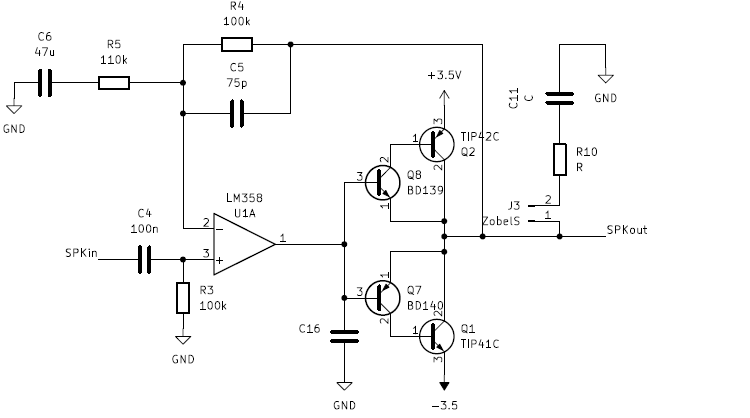
\includegraphics[width=0.7\textwidth]{images/2/2-2/circuitoAmplificadorAltavoces.png}
    \caption{Circuito amplificador de altavoces}
    \label{fig:2-2-amp-altavoz}
\end{figure}

\subsubsection{Diseño de PCB}

Todos estos sistemas se han integrado en una única PCB para intentar maximizar la integridad de la señal de audio, lo cual se consigue totalmente si se conecta el circuito sin tener en cuenta el \autoref{subsec:entre-dos-tierras}.

Hemos utilizado conectores Jack hembra de 3.5 mm para las dos entradas de audio y la salida a los auriculares. Un problema de este tipo de conectores es que el número de anillos puede variar en función de si los auriculares tienen o no micrófono y si son mono o estéreo. Si se quiere utilizar unos auricules con micrófono con nuestro sistema, se deben dejar ligeramente extraidos del conector para que haga mejor contacto la banda de tierra y mejorar significativamente el sonido.

La salida de altavoz se realiza a través de un terminal de dos tornillos para facilitar su conexión.

Como ya hemos comentado anteriormente, el circuito de transistores cuenta con un condensador de estabilizacion que finalmente no hemos utilizado. 

Además, hemos añadido la posibilidad de utilizar una red de Zobel, circuito que sirve para linealizar la respuesta en frecuencia de la inductancia intrínseca de los altavoces mediante un capacitor y una resistencia, pero finalmente no la hemos necesitado, por lo que tampoco está soldada.

El circuito cuenta además con un potenciómetro que sirve para ajustar el offset de la tensión de la tierra virtual gracias a los terminales específicos del \texttt{OP07}.

Hemos utilizado componentes SMT para los componentes pasivos y los conectores de audio y THT para los circuitos integrados, transistores y conectores de terminal.

Se puede ver una imagen del circuito finalizado en la \autoref{fig:2-2-circuito-foto} y el esquemático completo en el \autoref{anexo:circuito-audio}.

\begin{figure}[h]
    \centering
    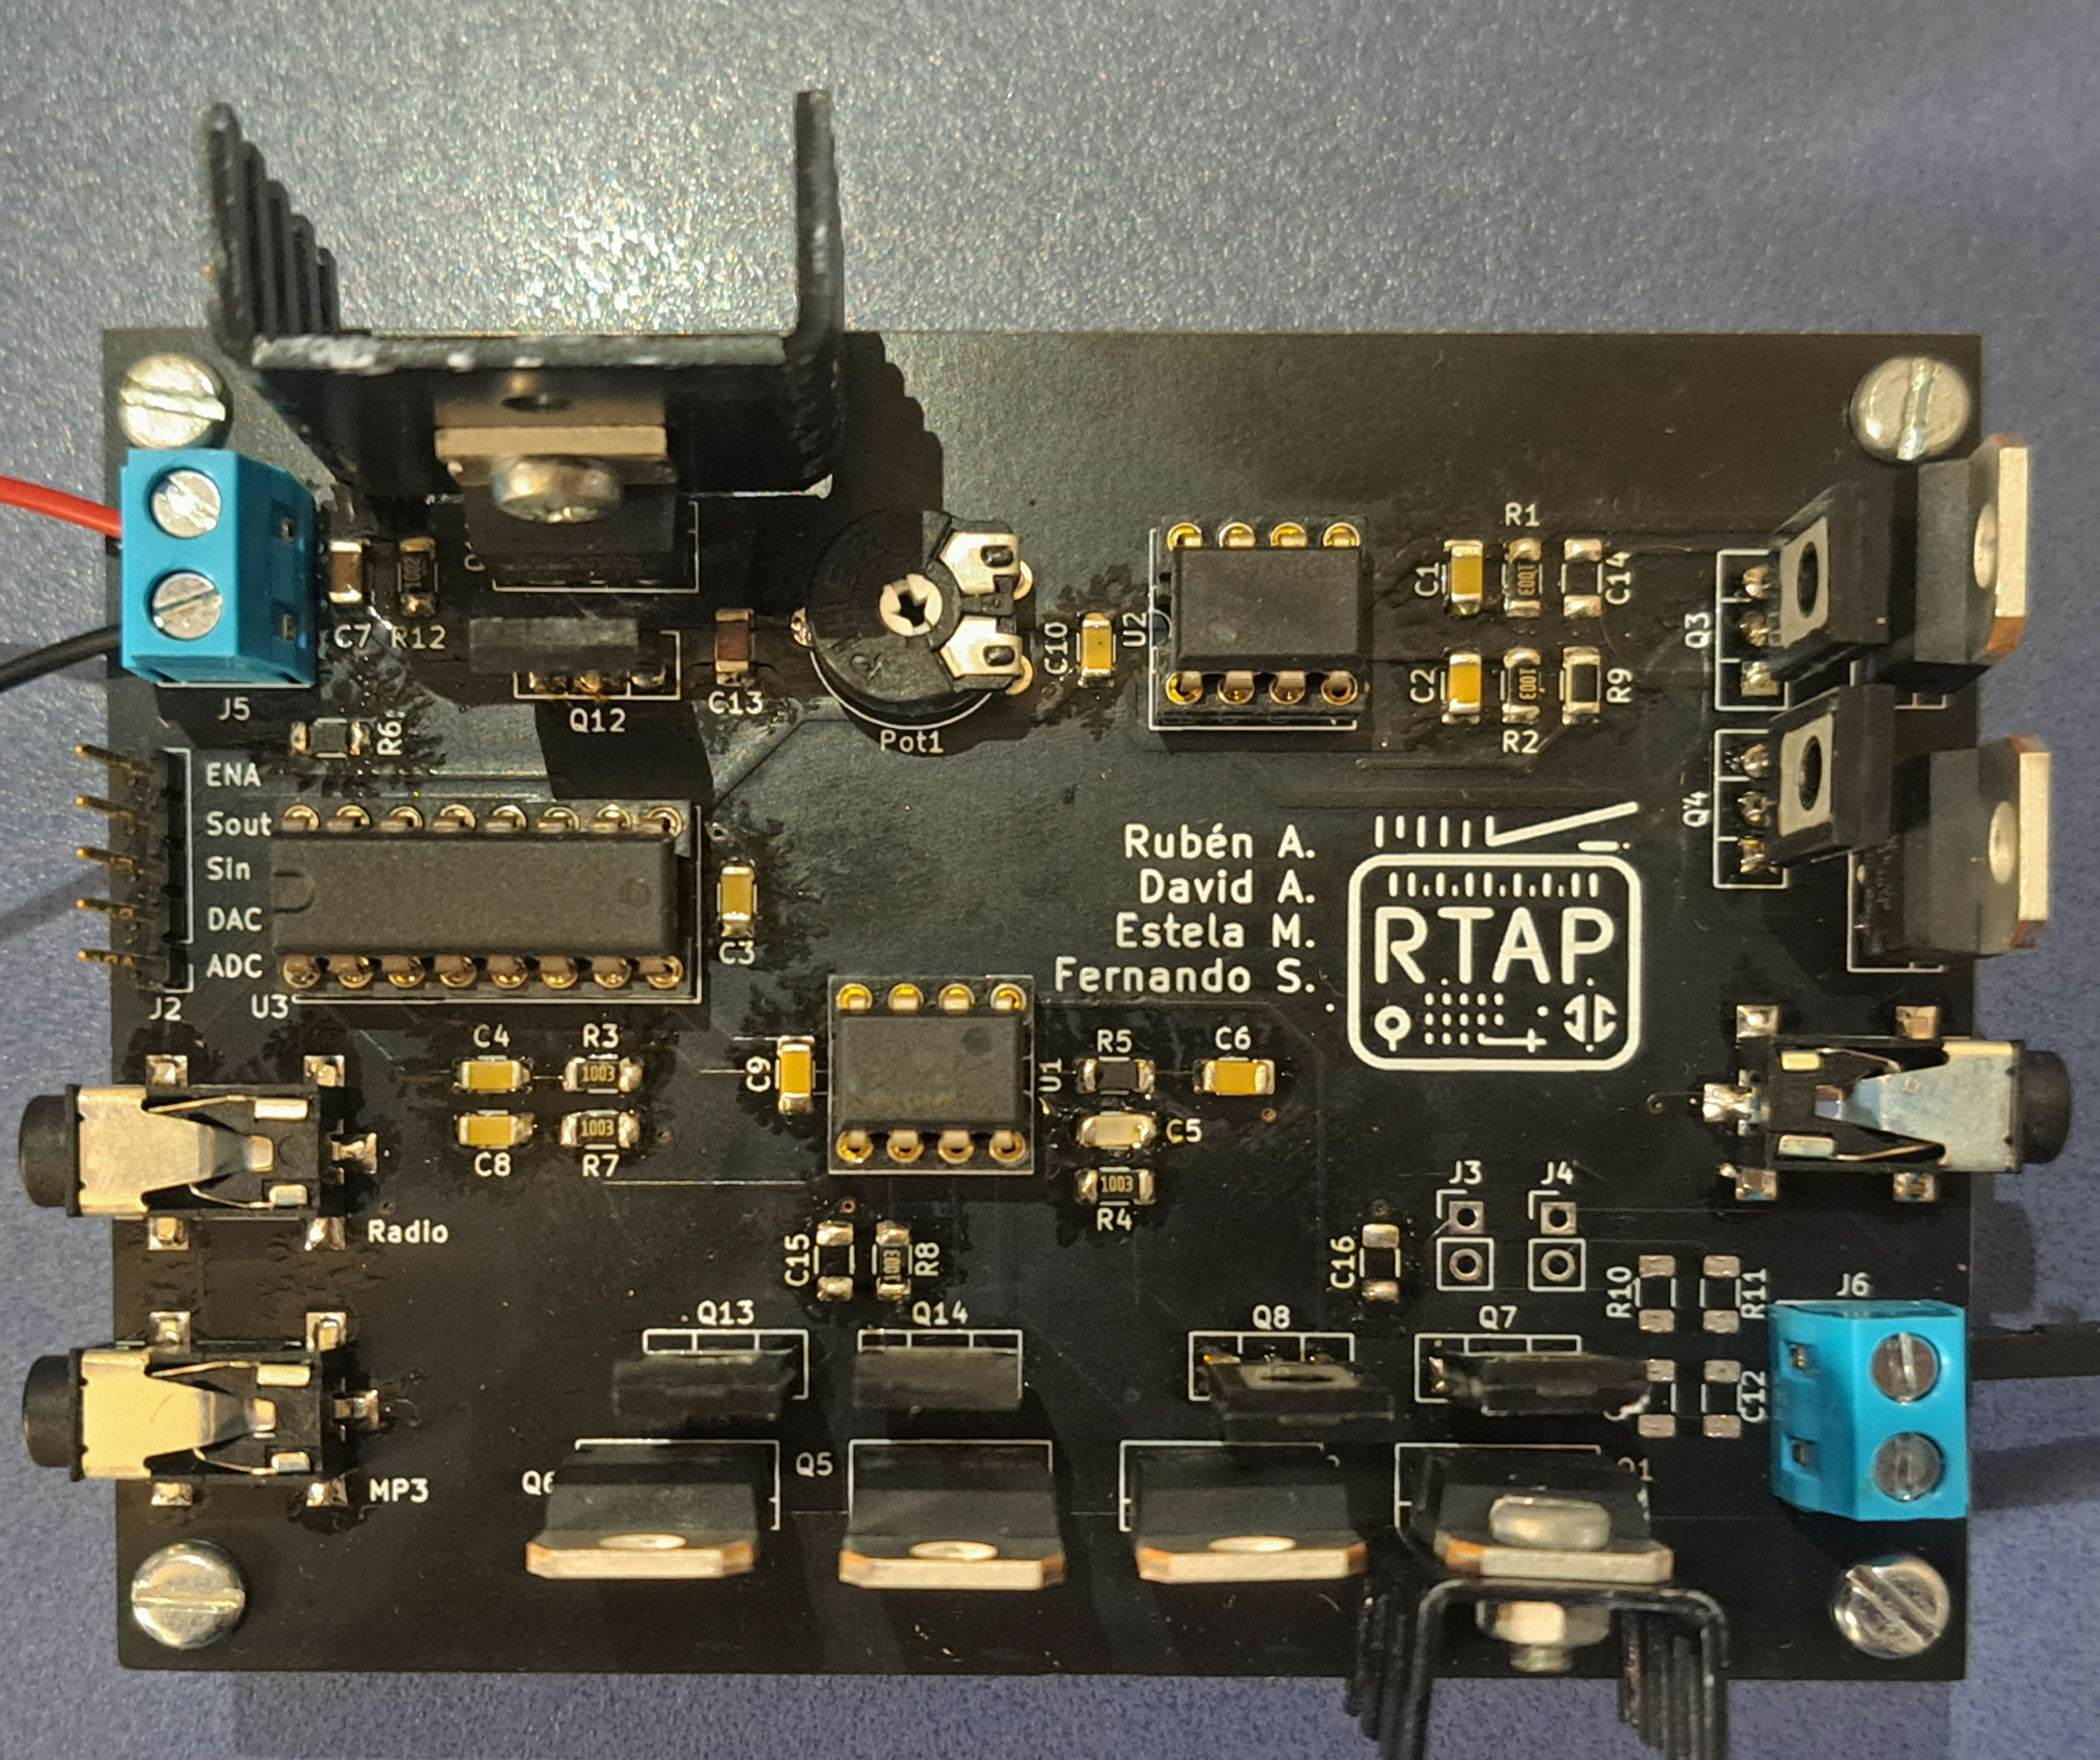
\includegraphics[width=0.5\textwidth]{images/2/2-2/circuito-foto.jpg}
    \caption{Circuito de audio completo}
    \label{fig:2-2-circuito-foto}
\end{figure}